%%%%%%%%%%%%%%%%%%%%%%%%%%%%%%%%%%%%%%%%%
% University/School Laboratory Report
% LaTeX Template
% Version 3.1 (25/3/14)
%
% This template has been downloaded from:
% http://www.LaTeXTemplates.com
%
% Original author:
% Linux and Unix Users Group at Virginia Tech Wiki 
% (https://vtluug.org/wiki/Example_LaTeX_chem_lab_report)
%
% License:
% CC BY-NC-SA 3.0 (http://creativecommons.org/licenses/by-nc-sa/3.0/)
%
%%%%%%%%%%%%%%%%%%%%%%%%%%%%%%%%%%%%%%%%%

%----------------------------------------------------------------------------------------
%	PACKAGES AND DOCUMENT CONFIGURATIONS
%----------------------------------------------------------------------------------------

\documentclass{article}

\usepackage{array}
\usepackage{tabularx}
\usepackage{graphicx} % Required for the inclusion of images
\usepackage[utf8]{inputenc}
\usepackage[english]{babel}
\usepackage{minted}
\usemintedstyle{borland}
\usepackage{xcolor}
\setlength\parindent{1.2pt} % Removes all indentation from paragraphs

\renewcommand{\labelenumi}{\alph{enumi}.} % Make numbering in the enumerate environment by letter rather than number (e.g. subsection 6)

%\usepackage{times} % Uncomment to use the Times New Roman font

%----------------------------------------------------------------------------------------
%	DOCUMENT INFORMATION
%----------------------------------------------------------------------------------------

\title{
	Microcontroller Lab Report \\
\large 8086 programming Part 1
} % Title

\author{
	Aaditya Prakash Kattekola \\
	{\small Roll: 194201} \\
	{\small ECE Section B} \\
} % Author name

\date{\today} % Date for the report

\begin{document}

\maketitle % Insert the title, author and date

% If you wish to include an abstract, uncomment the lines below
% \begin{abstract}
% Abstract text
% \end{abstract}


%----------------------------------------------------------------------------------------
%	Question x
%----------------------------------------------------------------------------------------

\break
\section{Question X}
%----------------------------------------------------------------------------------------
%	subsection 1
%----------------------------------------------------------------------------------------

\subsection{Aim}


%----------------------------------------------------------------------------------------
%	subsection 2
%----------------------------------------------------------------------------------------

\subsection{Program}
\subsubsection{Code}
\inputminted{nasm}{"C:/Users/aadit/Documents/BTech/5th Semester/MC Lab/Sample Lab Report/First.asm"}

\subsubsection{Emulator}

\begin{center}
\begin{tabularx}{1.0\textwidth} { 
  | >{\centering\arraybackslash}X 
  | >{\centering\arraybackslash}X 
  | >{\centering\arraybackslash}X | }
 \hline
\textbf{Address  (CS:0100, IP:0000)} &\textbf{Machine code}&\textbf{Instruction} \\
  \hline
 01000 & B8,00,21 & MOV AX, 02100H \\ 
  \hline
  & &  \\ 
  \hline
  & &  \\ 
  \hline
\end{tabularx}
\end{center}

%----------------------------------------------------------------------------------------
%	subsection 3
%----------------------------------------------------------------------------------------
\break
\subsection{Result}
\subsubsection{Input}
AX: 2100H \\
BX: 2800H \\

\subsubsection{Expectation}
AX $\leftarrow$ AX+BX; \\  
2100H+2800H $\rightarrow$ 4900H$\rightarrow$AX \\

%----------------------------------------------------------------------------------------
%	subsection 4
%----------------------------------------------------------------------------------------

\subsubsection{Emulator}

\begin{figure}[h]
\begin{center}
%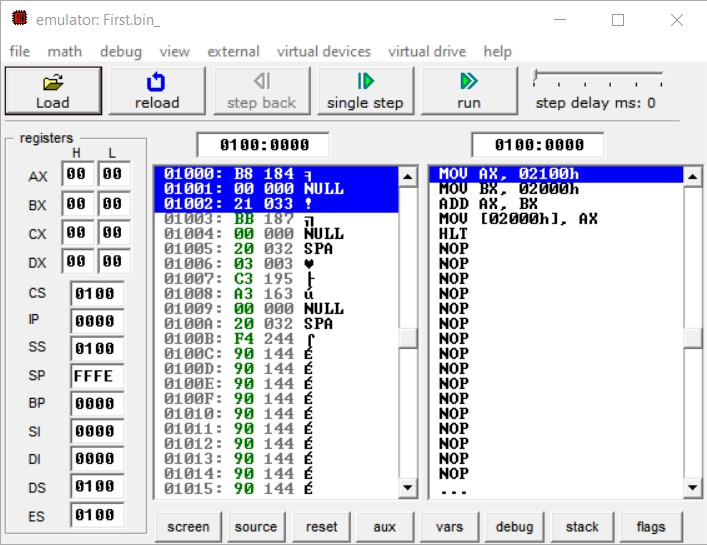
\includegraphics[width=1.0\textwidth]{output} 
\caption{Emulator Output}
\end{center}
\end{figure}




\end{document}